
%(BEGIN_QUESTION)
% Copyright 2006, Tony R. Kuphaldt, released under the Creative Commons Attribution License (v 1.0)
% This means you may do almost anything with this work of mine, so long as you give me proper credit

Consider this control system, set up to maintain the temperature of a chemical reactor vessel at a constant (``setpoint'') value.  The reactor's source of heat is a steam ``jacket'' where hot steam is admitted through a motor-operated (M) control valve (TV) according to the temperature inside the reactor sensed by the temperature transmitter (TT):

$$\includegraphics[width=15.5cm]{i00139x01.eps}$$

While doing some clean-up work near the reactor, you receive a frantic call from the operator on your two-way radio.  He says that the controller (TIC) is registering a temperature of 186 $^{o}$F, which is 11 degrees higher than the setpoint of 175 $^{o}$F.  A temperature this high could ruin the product inside the reactor.  He wants you to check the temperature indicator on the side the reactor (TI) and let him know what it reads.

You look at the TI, and see that it registers a temperature of 172 $^{o}$F, which is a bit too cold if anything, not too hot.  You immediately report this to the operator using your radio, who then asks you to check out the system to see why he's getting a false reading on the controller display.

Fortunately, you have your multimeter and tool set with you, so you proceed to the temperature transmitter to measure the milliamp signal it is outputting.  Removing a cover from a round junction box on the conduit where the transmitter's wires are routed, you see a terminal block inside with a 1N4001 rectifying diode placed in series with the circuit:

$$\includegraphics[width=15.5cm]{i00139x02.eps}$$

Setting your multimeter to measure milliamps, you connect the red and black test leads across the diode.  This shorts past the diode, forcing all the current to go through the meter instead of the diode, allowing you to ``break in'' to the 4-20 mA circuit without having to physically break a wire connection anywhere.  Making a mental note to thank your instrumentation instructor later for showing you this trick, you see that your multimeter registers 15.683 mA.

Given a calibrated temperature transmitter range of 100 to 200 degrees F, determine what this current measurement tells you about the location of the problem in this temperature control loop, and explain how you made that determination.

\vskip 20pt \vbox{\hrule \hbox{\strut \vrule{} {\bf Suggestions for Socratic discussion} \vrule} \hrule}

\begin{itemize}
\item{} Why is it important for technicians to be able to easily convert milliamp signal values into corresponding process variable (PV) values?
\item{} How does the diode perform this useful function of allowing current measurement without breaking the circuit?
\item{} Supposing there were no diode in this loop circuit, how would you suggest we measure the transmitter's output current?
\item{} Is it possible that the fault in this system could be something to do with the control valve?  Why or why not?
\end{itemize}

\underbar{file i00139}
%(END_QUESTION)





%(BEGIN_ANSWER)


%(END_ANSWER)





%(BEGIN_NOTES)

The problem most likely lies within the controller (TIC).

\vskip 10pt

The calculation for temperature based on the milliamp measurement taken and the known range of the temperature transmitter is as follows:

$$\left({15.683 \hbox{mA} - 4 \hbox{ mA}} \over 16 \hbox{ mA}\right) \times 100 \hbox{ deg F} + 100 \hbox{ deg F} = 173.02 \hbox{ deg F}$$

To summarize, we take the measured current and subtract the live zero offset (4 mA), then divide by the span of the milliamp signal range (16 mA).  This yields a fractional value representing 0 to 100 percent of measurement range.  Multiplying this fractional value by the span of the measurement range (200 deg F $-$ 100 deg F = 100 deg F) and lastly adding the zero offset of the measurement range (100 deg F) tells us the process temperature as interpreted by the transmitter, which in this particular case is 173.02 deg F.

This measured value is so close to the value of 172 deg F reported by the temperature gauge that we may safely conclude the transmitter is functioning properly.  This means something {\it else} must account for the controller's abnormal temperature reading.  In other words, the transmitter is fine but the controller is falsely interpreting the 15.683 mA signal to mean a significantly higher temperature.

A couple of possibilities are as follows: perhaps the analog-to-digital converter circuitry inside the controller is faulty, causing the 4-20 mA current signal to be converted into an incorrect numerical value in degrees F.  Alternatively, the resistor located on the controller for converting the 4-20 mA signal into a voltage drop for the analog-to-digital converter to read may be faulty, or have a loose wire connection to the controller's terminal (adding extra resistance to the 4-20 mA loop and causing an excessive voltage drop which is then interpreted by the controller as a too-high temperature).  Whichever the case, we know the transmitter is not at fault!

%INDEX% Basics, control loop troubleshooting: determining cause of control problem
%INDEX% Process: steam-heated reactor vessel (generic)

%(END_NOTES)


